\documentclass[border=5pt]{standalone}
% Style commun aux figures de structure de MPMbox
% ------------------------------------------------
\usepackage[utf8]{inputenc}
\usepackage[T1]{fontenc}
\usepackage[english]{babel}
\usepackage{lmodern}
\usepackage{tikz}
\usetikzlibrary{positioning,arrows.meta,calc,fit,backgrounds,shapes.geometric}
% babel(french) rend « : » actif, ce qui casse les coordonnées polaires (90:4cm)
\usetikzlibrary{babel}

% pas de césure dans les boîtes étroites
\hyphenpenalty=10000
\exhyphenpenalty=10000
\tolerance=9999
\emergencystretch=3em

\definecolor{mpmBase}{HTML}{1F3A5F}    % classes de base
\definecolor{mpmBaseBg}{HTML}{E8EEF6}
\definecolor{mpmDeriv}{HTML}{4A7BA7}   % variantes
\definecolor{mpmDerivBg}{HTML}{F5F8FB}
\definecolor{mpmData}{HTML}{7A5230}    % données simulées
\definecolor{mpmDataBg}{HTML}{FBF3E8}
\definecolor{mpmAccent}{HTML}{A6432F}  % mise en avant (MPMxDEM)
\definecolor{mpmAccentBg}{HTML}{FBEEEB}
\definecolor{mpmGrey}{HTML}{5A6472}

\tikzset{
  base/.style={
    draw=mpmBase, line width=0.9pt, fill=mpmBaseBg, rounded corners=3pt,
    text width=#1, align=center, inner sep=6pt, font=\sffamily\small},
  base/.default=5.2cm,
  deriv/.style={
    draw=mpmDeriv, line width=0.6pt, fill=mpmDerivBg, rounded corners=2pt,
    text width=#1, align=left, inner sep=5pt, font=\sffamily\scriptsize},
  deriv/.default=7.4cm,
  data/.style={
    draw=mpmData, line width=0.7pt, fill=mpmDataBg, rounded corners=3pt,
    text width=#1, align=center, inner sep=5pt, font=\sffamily\scriptsize},
  data/.default=4.2cm,
  accent/.style={
    draw=mpmAccent, line width=0.8pt, fill=mpmAccentBg, rounded corners=2pt,
    text width=#1, align=left, inner sep=5pt, font=\sffamily\scriptsize},
  accent/.default=7.4cm,
  spine/.style={draw=mpmDeriv, line width=0.6pt},
  link/.style={draw=mpmGrey, line width=0.6pt, -{Stealth[length=4pt]}},
  dashlink/.style={draw=mpmGrey, line width=0.6pt, densely dashed,
                   -{Stealth[length=4pt]}, font=\sffamily\tiny},
  mpmcap/.style={font=\sffamily\scriptsize\itshape, text=mpmGrey},
}

% Titre d'une classe de base : \classname{Nom}{rôle}
\newcommand{\classname}[2]{{\bfseries #1}\\[2pt]{\scriptsize\itshape #2}}
% Ligne d'une variante : \variant{Nom}{description}
\newcommand{\variant}[2]{{\bfseries\ttfamily #1}\quad #2}

\begin{document}
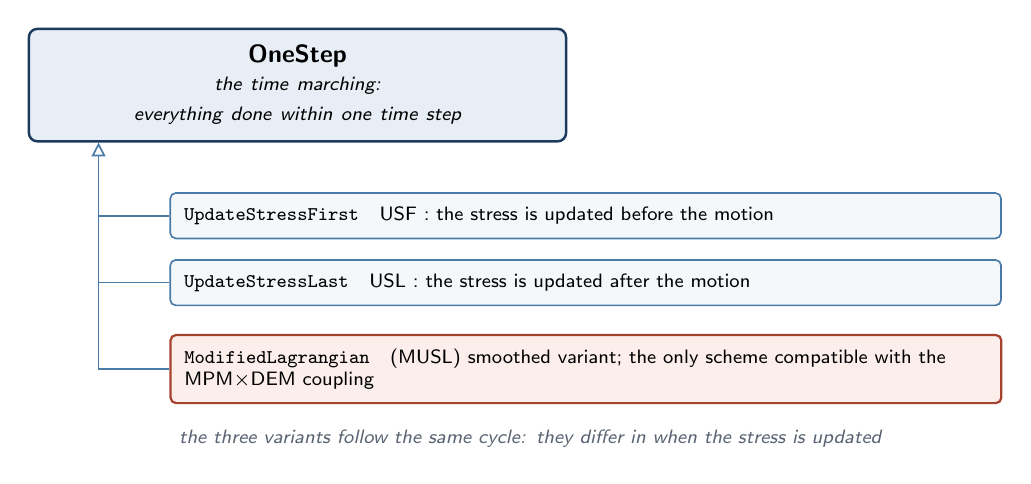
\begin{tikzpicture}

\node[base=6.4cm, anchor=north west] (B) at (0,0)
  {\classname{OneStep}{the time marching:\\ everything done within one time step}};

\coordinate (S) at ($(B.south west)+(0.9cm,-0.40cm)$);
\draw[spine,-{Triangle[open,fill=white,length=5pt,width=5pt]}] (S) -- ($(B.south west)+(0.9cm,0)$);

\foreach \nm/\ds [count=\i] in {%
  UpdateStressFirst/{USF} : the stress is updated before the motion,
  UpdateStressLast/{USL} : the stress is updated after the motion%
} {
  \node[deriv=10.2cm, anchor=north west] (D\i) at ($(S)+(0.9cm,-0.85cm*\i+0.62cm)$)
    {\variant{\nm}{\ds}};
  \draw[spine] (S) |- (D\i.west);
}

\node[accent=10.2cm, anchor=north west] (D3) at ($(S)+(0.9cm,-0.85cm*3+0.52cm)$)
  {\variant{ModifiedLagrangian}{(MUSL) smoothed variant; the only scheme
   compatible with the MPM$\times$DEM coupling}};
\draw[spine] (S) |- (D3.west);

\node[mpmcap, anchor=north west, text width=9.0cm] at ($(D3.south west)+(0,-0.2cm)$)
  {the three variants follow the same cycle: they differ in when the stress
   is updated};

\end{tikzpicture}
\end{document}
